\noindent\section*{Introduction}
Quality Threshold (QT) clustering is an algorithm originally created to perform gene clustering. The goal of the algorithm is to find quality clusters. The clustering process is started with the maximum diameter of a cluster instead of the K number of clusters like in other algorithms, e.g. K-means clustering. \cite{Heyer, Jin}  \\

\noindent In the context of genomics, after expression levels have been determined the goal is to find similar expression patterns - meaning that the genes are co-expressed. A score to compare the genes has to be computed. It can be, for example a similarity score. After this, the clustering can be performed. \cite{Heyer} \\

\noindent The goal of this project is to make a Julia language (version 1.5.0) program with the QT clustering algorithm. The ultimate goal of the program is to perform faster and more efficiently than the same algorithm programmed in Python or Perl. 

\noindent\section*{Algorithm}
The algorithm follows very simple steps, (1) Starts by forming \textit{candidate clusters}, so finding points that are closer than a threshold. Usually as input, there is a threshold or a percentage of the maximum diameter, so the threshold will be $threshold = max\_diameter \frac{x}{100}$. The points, that increase the cluster diameter the least and that this distance is not larger than the threshold, are continuously added to the cluster. \\ 

\noindent One of the advantages of this type of clustering is that it guarantees that the best clusters are obtained and there are no prior knowledge requirements. The "disadvantage" is that the first version of the algorithm is computationally expensive ($O(N^3)$), however, in this project there are shown some optimizations that lower the computation time and the cluster will end up being fast and efficient.

\section*{Optimizations}
\noindent As mentioned before, the algorithm has a high computational cost. To reduce the running time of the algorithm. We propose several optimizations: building a distance matrix between each of the points, calculation of candidates before starting the clustering, re-calculation of clusters after one cluster has been selected and continuously checking if any of the current clusters has been already calculated. Moreover, some language specific optimizations can be performed. \\

\noindent \textbf{Distance Matrix}\\
\noindent This simple optimization is nothing more than building a pairwise distance matrix between each of the data points in the beginning so the calculation is not to be repeated over the algorithm.

\begin{verbatim}
matrix = m,n
for i in  m
  for j in n
    if i != j or i > j 
     euclidean distance for (data[i],
     data[j])
     fill matrix[i,j]
\end{verbatim}

\noindent \textbf{Calculation of candidate points}\\
\noindent Instead of building the clusters every time to find which are the points that are within the threshold or QT distance, a calculation of candidate points can be performed. Calculation of candidate points means that for each \textit{origin} point, the points surrounding it within the QT distance are put in a \textit{pre-candidate cluster}. As shown in figure \ref{fig:candidate_points}, the red points configure the candidate points for the original blue point. Only those red points will be taken into account when building a the first candidate cluster for the blue point. 

\begin{verbatim}
for i in num_points
  for j in num_points
    if i != j and distance_matrix[i,j]
    < threshold
        append j to candidate_points[i]
\end{verbatim}

\begin{figure}[h]
    \centering
    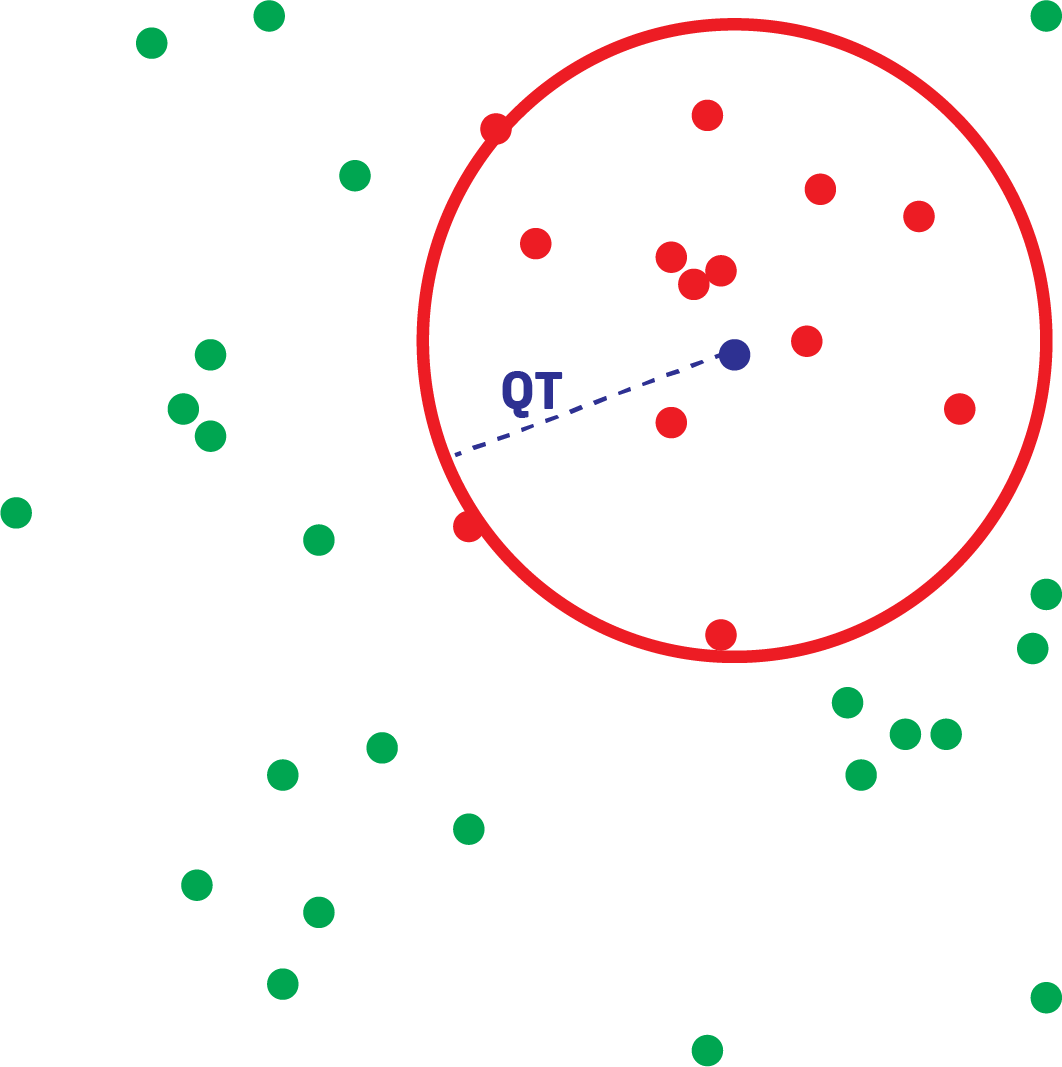
\includegraphics[width=0.4\textwidth]{images/CANDIDATE.png}
    \caption{\textbf{Candidate Points Representation}. Blue: origin point, red: candidate points, green: out of QT distance points.}
    \label{fig:candidate_points}
\end{figure}

\noindent \textbf{Recalculation of clusters}\\
Once the candidate points have been calculated and the QT clustering itself is started,  the algorithm occurs inside a \textit{while loop} that will finish when no points are left to put in a cluster. \\

\noindent Inside the \textit{while loop}, is where the \textit{candidate clusters} are obtained. After obtaining the first array of \textit{candidate clusters}, the \textit{top cluster}r is selected. This \textit{top cluster} must meet one of the following conditions:

\begin{enumerate}
    \item Select the cluster with more points.
    \item If condition \#1 is met by two or more \textit{candidate clusters}. Select the cluster with the smallest diameter, or what is the same, the cluster with the highest cluster density. 
    \item If condition \#1 and \#2 are met by two or more \textit{candidate clusters}. Select the candidate cluster arbitrarily. For example, select the candidate cluster where the index of its points is smaller regarding the input file.
\end{enumerate}

\noindent Once the top cluster, the \textit{Recalculation of candidate clusters} optimization is called. This optimization will compute the clusters again taking into account the \textit{points} that are left after subtracting the points from the \textit{top cluster}. This optimization makes sure that the \textit{candidate clusters} are not calculated for the points that have already been selected as a cluster for the final result. Moreover, in this optimization the only \textit{candidate clusters} that will be recalculate are from the points that were at QT distance from the points in the \textit{top cluster}. Because there are some points, as shown in figure \ref{fig:candidate_points}, the blue dots are forming a \textit{top cluster} and the points that are in red will be the only ones the algorithm needs to recalculate the candidate clusters for. With this, the number of calculations to do at each iteration becomes lower. 

\begin{verbatim}
for point in output_clusters
   append to aggregate: clusters of 
   top_cluster points

remove top cluster from aggregate
	
empty clusters of top_cluster points

check differences in cluster[point] and 
  cluster[top_cluster points]
if false
   empty cluster[point]
\end{verbatim}

\begin{figure}[h]
    \centering
    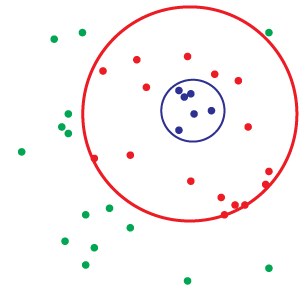
\includegraphics[width=0.4\textwidth]{images/CANDIDATE_2.png}
    \caption{\textbf{Recalculation of candidate clusters}. Blue: top cluster, red: points QT distance from the top cluster points that need to recalculate their candidate clusters, green: out of QT distance points.}
    \label{fig:candidate_clusters}
\end{figure}

\noindent \textbf{Check for existing clusters}\\
The last algorithm optimization is checking for existing clusters. This is done in the step where the candidate clusters from the candidate points are calculated. When calculating the candidate clusters, at $x$ iteration there will be a check on the already created clusters. In the program here, it is followed the Fibonacci's series, so there will be a check of clusters at $x = 2,3,5,8,...$.\\

The optimization applied here checks if the length of the \textit{current cluster} is present in the Fibonacci's series, if $true$ the \textit{current cluster} points are sorted and transformed to a dictionary key. Then it checks if the key exists in the dictionary and if $true$ it returns it together with the cluster diameter, if it does not exist in the dictionary, it appends it together with the \textit{origin}, which in this case is the current cluster. 

\begin{verbatim}
if length(candidate_cluster) in fib
    key = sorted candidate_cluster
	if key in dict		
		return cluster and diameter
	add key, value to dict
\end{verbatim}

\noindent \textbf{Language Specific Optimizations}\\
Julia offers a vast variety of data structure and even the possibility for the user to create its own data structures. Due to this, the algorithm can even be more optimized and compute more efficiently some basic calculations such as the candidate points, the distance matrix or reading a simple input file with vectors. \\

\section*{Results}
% correct results 

In figure \ref{fig:all}, it is plotted all the data points together, from the 100 points provided data set. It is a non-informative plot because no special behaviours or trends can be distinguished. However, looking at figure \ref{fig:clusters}, it can be seen that QT clustering results show that the points that cluster together show a common trend. The clusters in the beginning are the ones that contain more points, whether the last points to cluster are left as singletons. \\ 
% show plots
\begin{figure}[h]
    \centering
    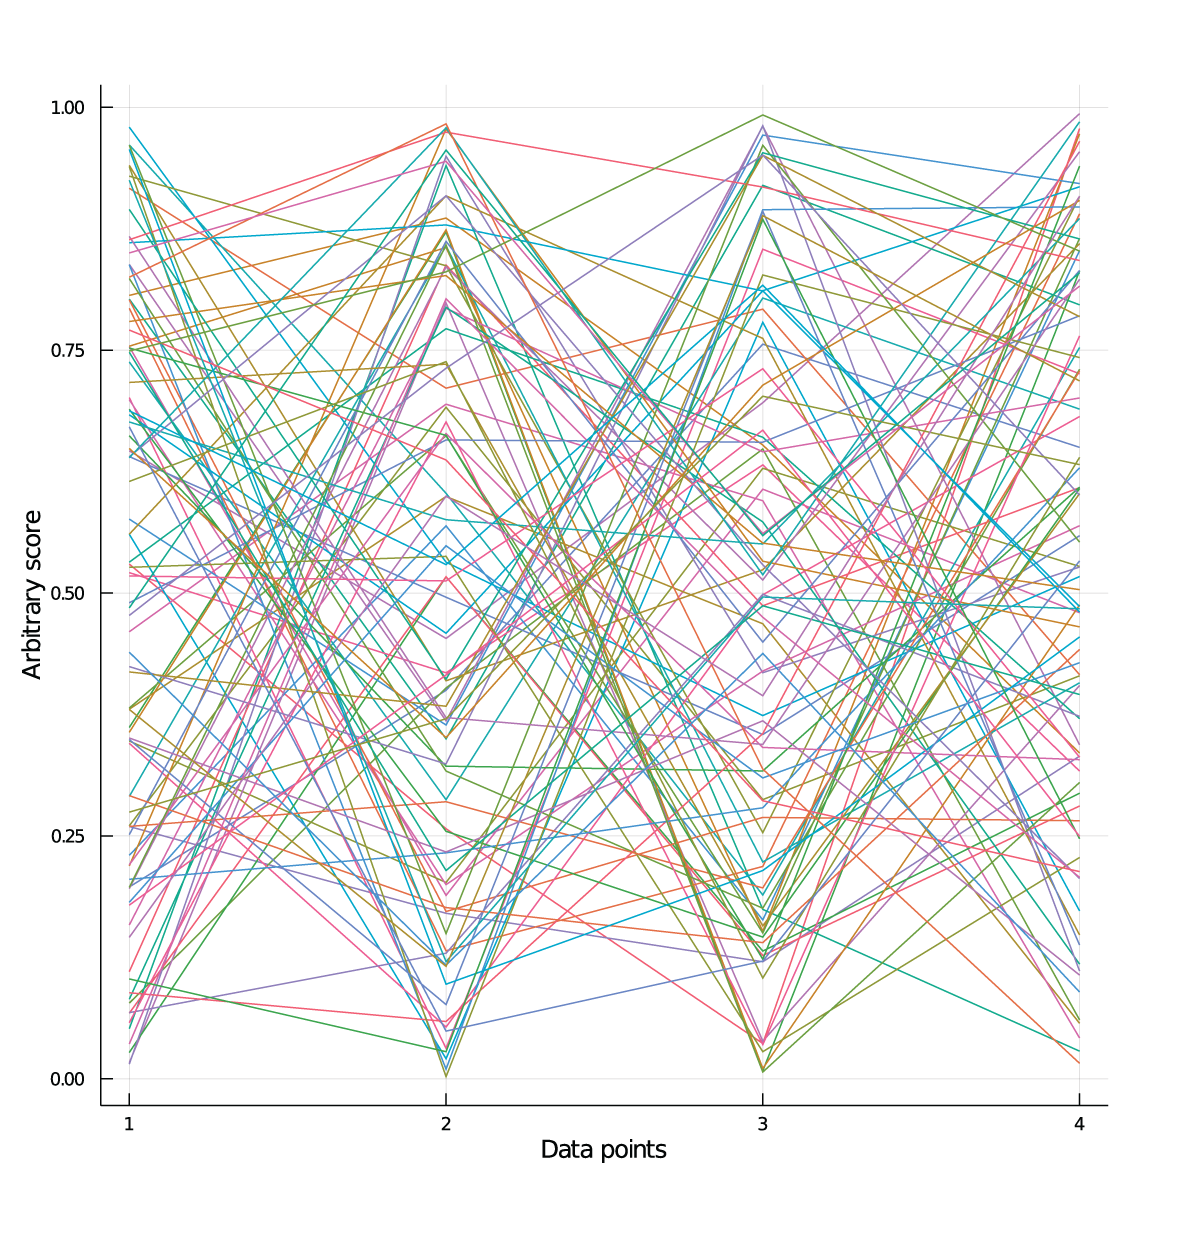
\includegraphics[width=0.4\textwidth]{images/myplot_initial.png}
    \caption{\textbf{All the data points plotted together}.}
    \label{fig:all}
\end{figure} 
\begin{figure}[h]
    \centering
    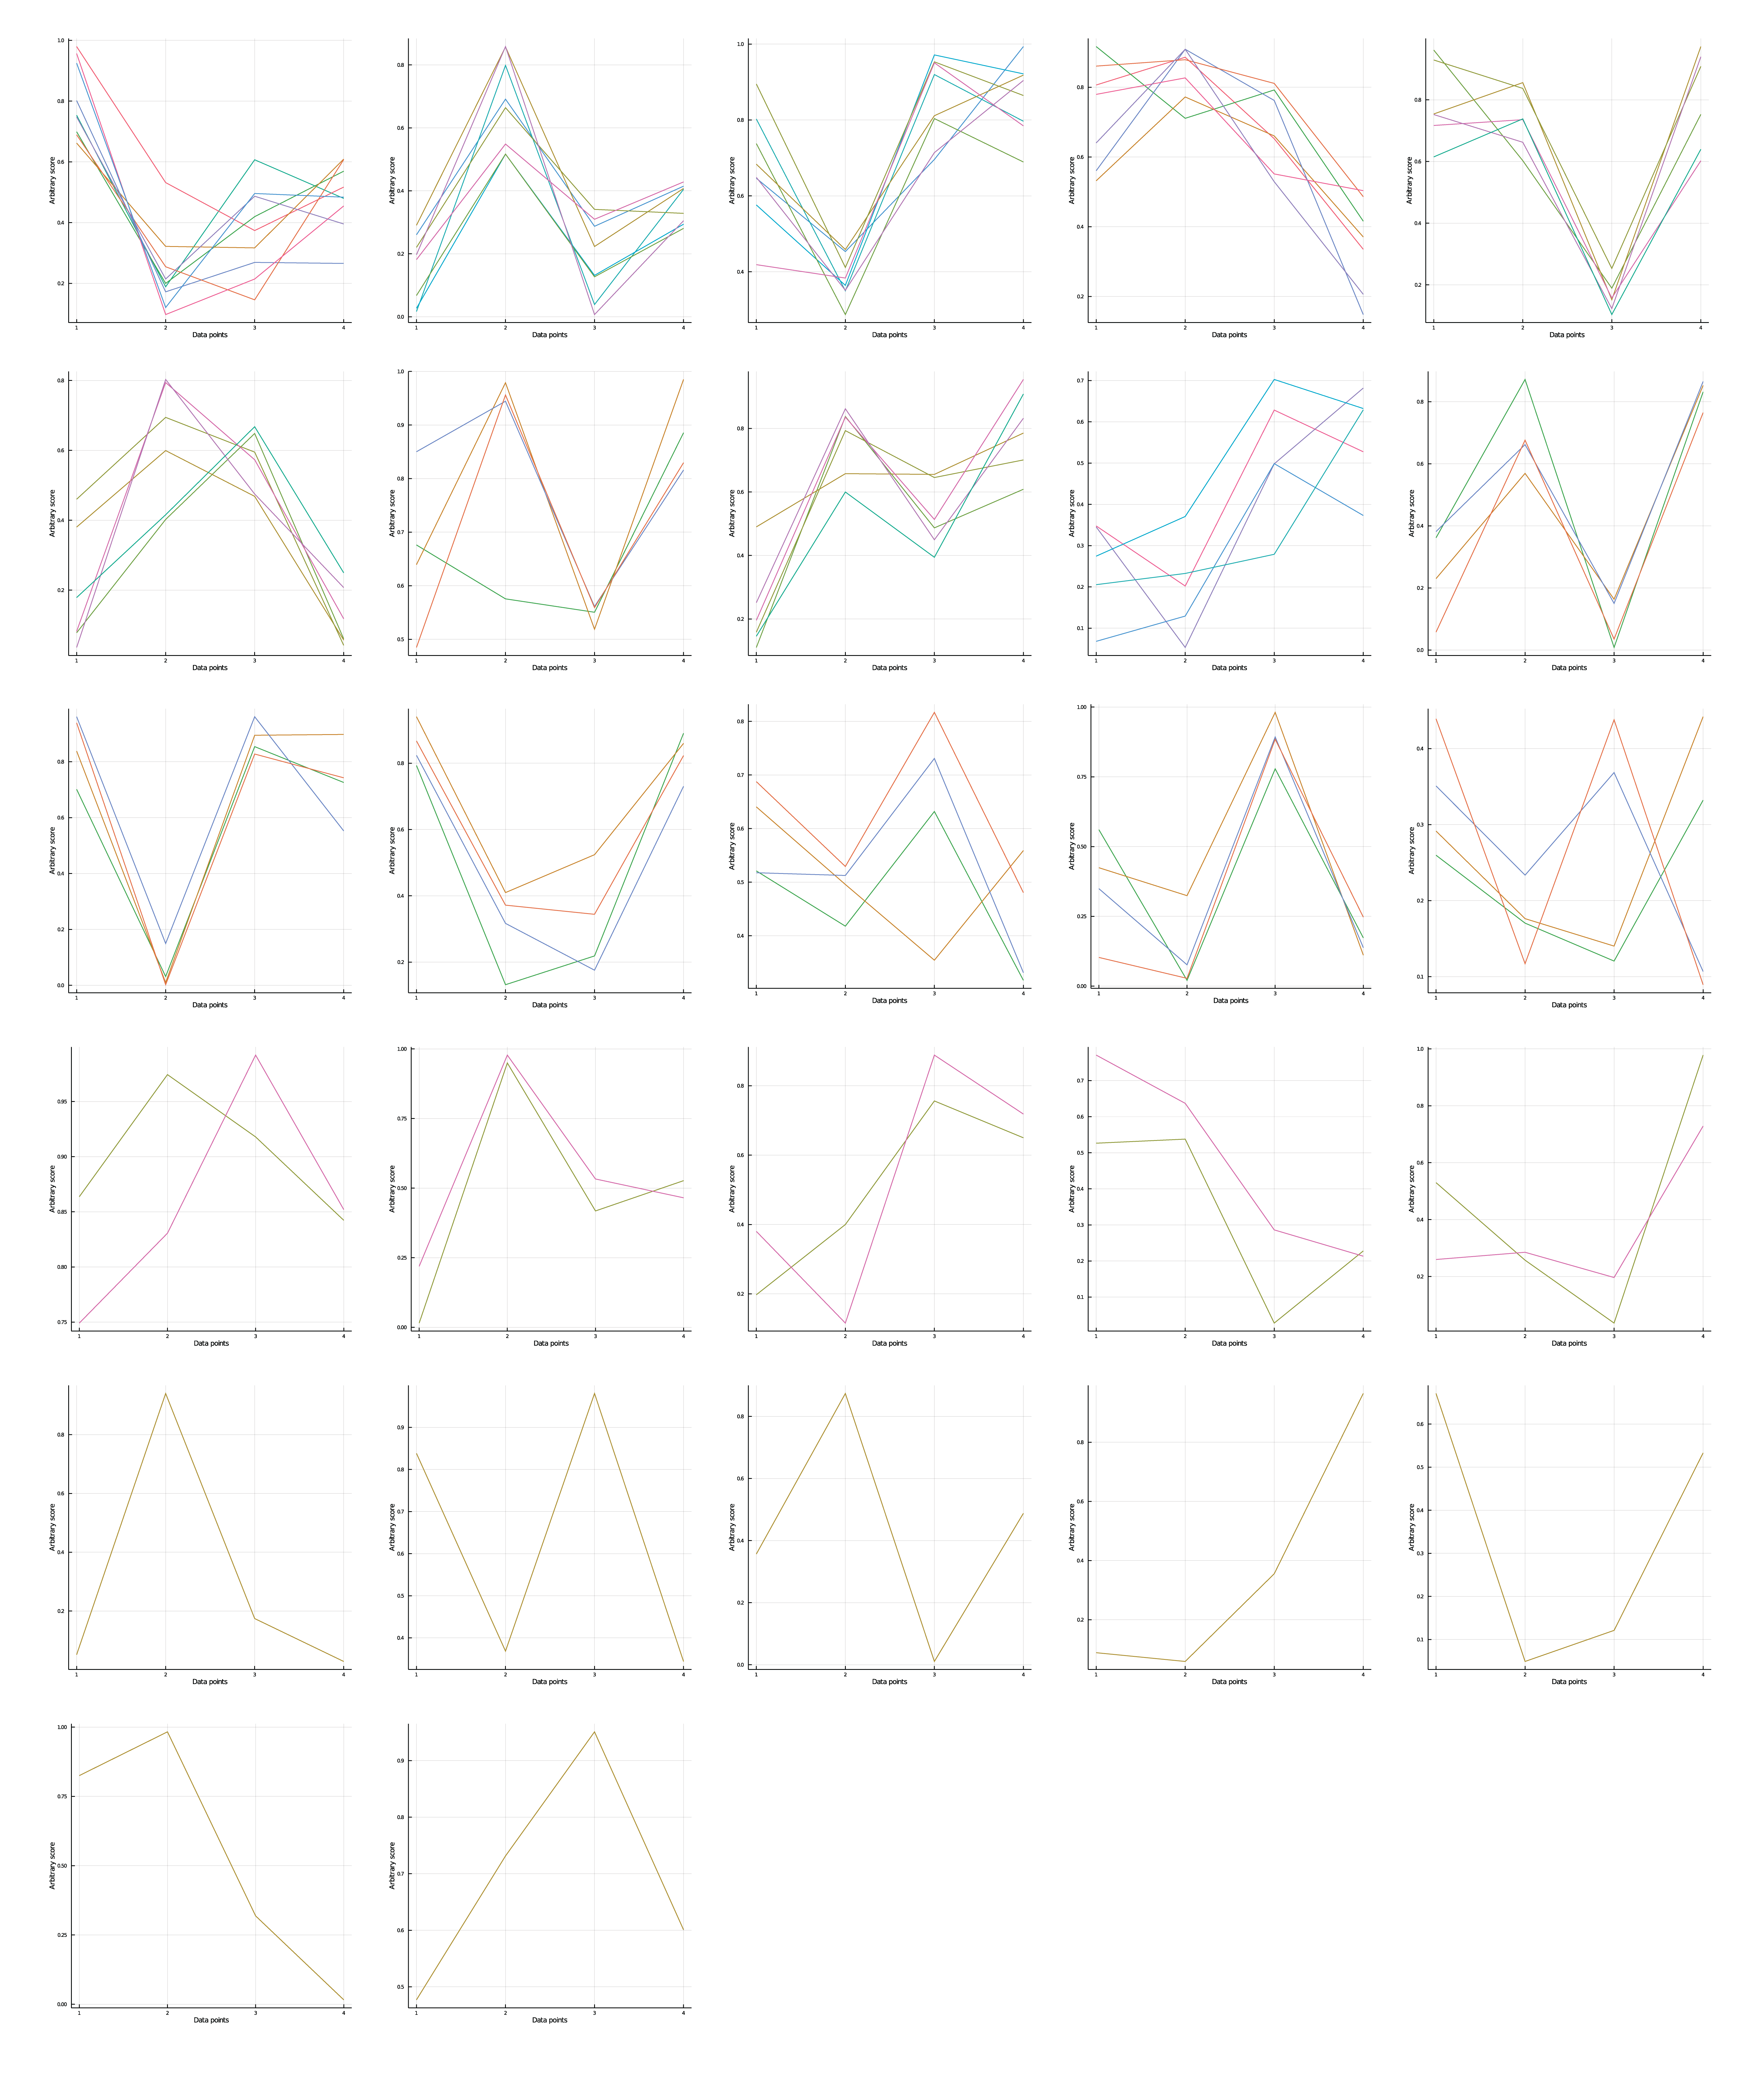
\includegraphics[width=0.5\textwidth]{images/clusters_separate.png}
    \caption{\textbf{All the clusters plotted separately}.}
    \label{fig:clusters}
\end{figure}

% show times
Looking at the performance of the algorithm programmed in Julia language and knowing that the same algorithm with the same optimizations in Python takes $\pm$ 6 minutes for 4169 points (original number of points from the original publication \cite{Heyer}). The present Julia program only takes an average of 75 seconds to cluster 4169 points. Being able to cluster 10,000 points in 650 seconds, see \ref{fig:time}. Finally, the code can be found at \href{https://github.com/laurasansc/learning_julia}{Julia Project Github Repository}. \\

\begin{figure}[h]
    \centering
    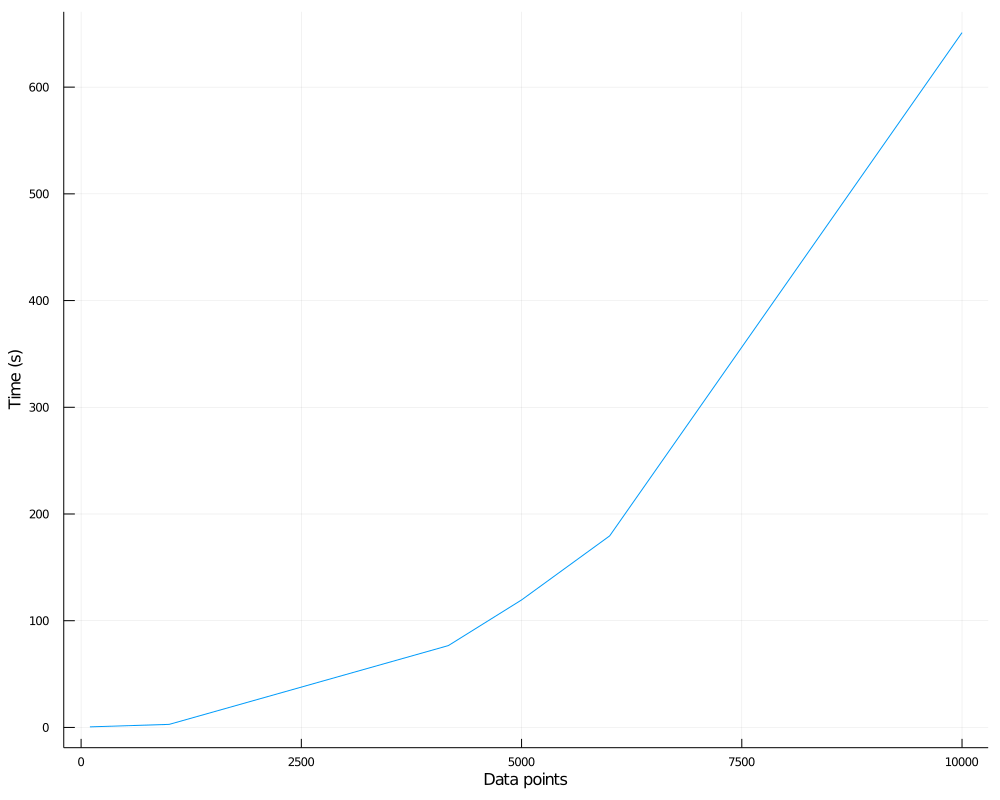
\includegraphics[width=0.5\textwidth]{images/times.png}
    \caption{\textbf{Running time for each data set of 100, 1000, 4169, 5000, 6000 and 10000 points}.}
    \label{fig:time}
\end{figure}

\section*{Conclusions}
To summarize, Julia has proven a more efficient computation of the QT clustering algorithm if compared to Python and Perl. However, the language specific optimizations have not been carried out. In further projects, there is still a lot of margin for the project to improve running time. 

